\documentclass[8pt]{article}
\usepackage{graphicx}
\usepackage[utf8]{inputenc}

\title{Temporally equitable subsidies: a two-phase token minting schedule}
\author{arjunhassard}
\date{Feb 2020}
\begin{document}
\maketitle


\section{Summary}

The previous draft of NuCypher's subsidy (inflationary reward) model commences with an annual inflation `rate' of 100\% at network launch. The genesis rate then decays with a half-life of 2 years – i.e. it drops by a factor of 2 every other year. For example, on day 200 of the network, the annual inflation rate would be approximately 83\%.

\begin{figure}[h!]
    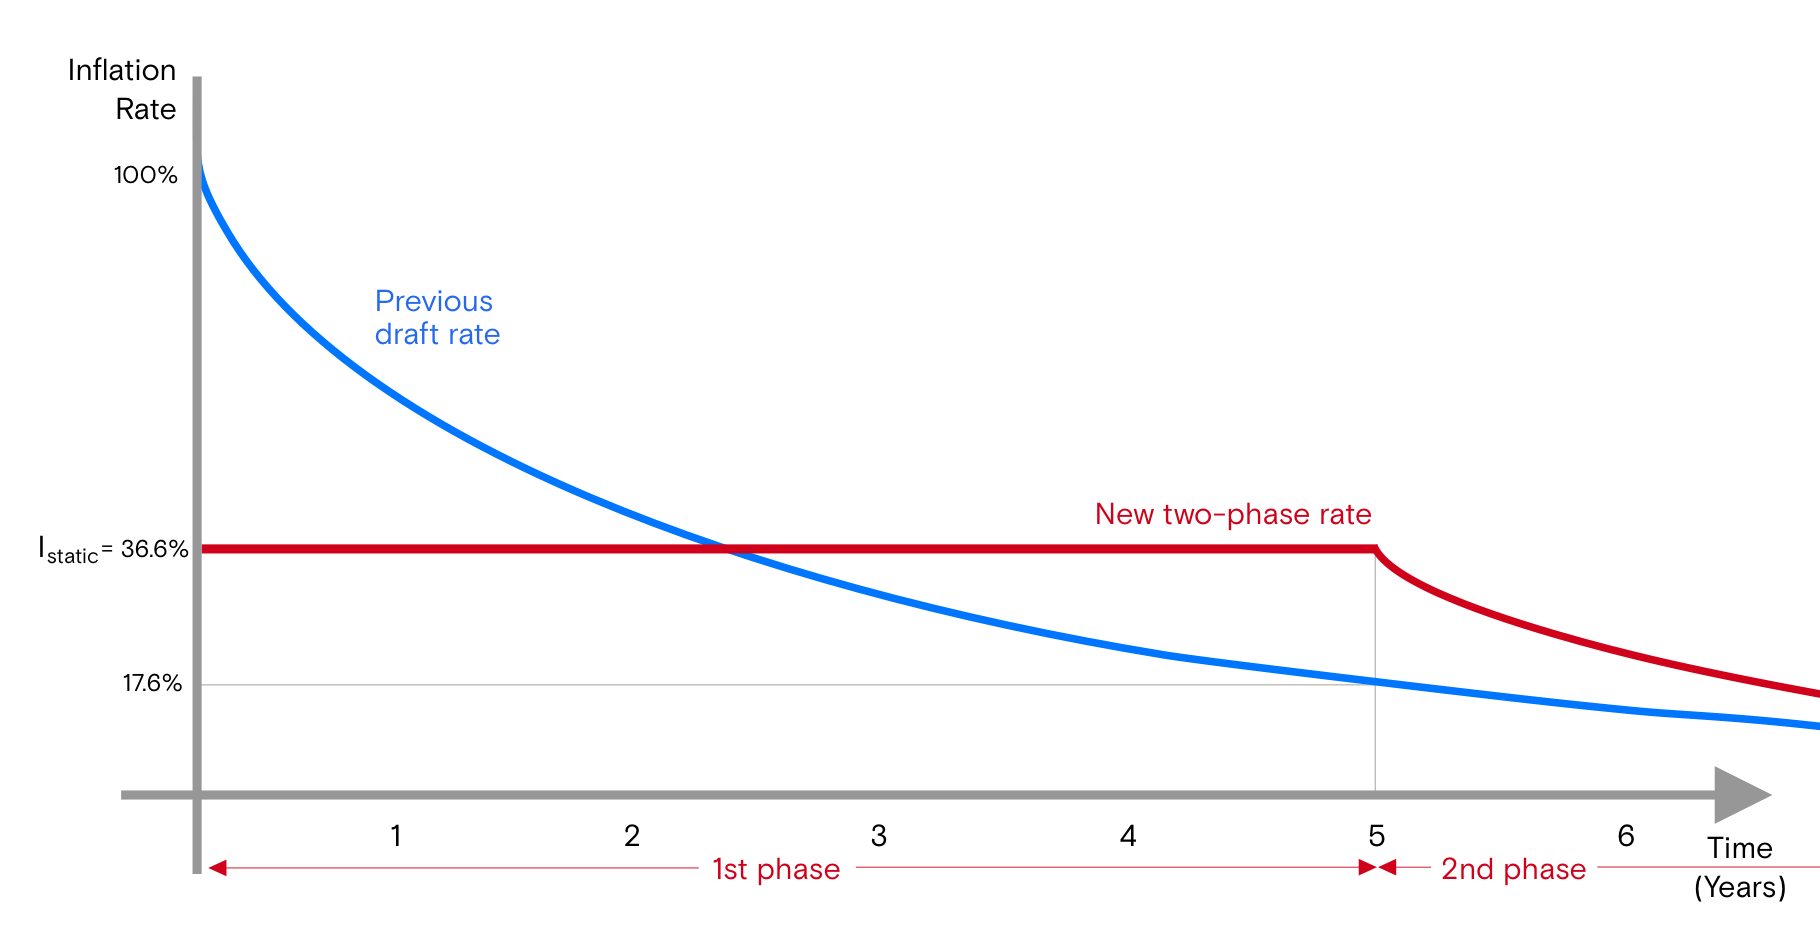
\includegraphics[width=\textwidth]{Two_phase_inflation.png}
    \caption{Illustration comparing the previous draft and two-phase model over the first 6 years of the network's lifetime.}
    \label{fig:tp}
\end{figure}

An alternative to the previous model is proposed here; a static (unchanging) inflation rate of \textbf{36.6\%} for the first 5 years, which implies the minting of approximately 366 million new tokens per year. From day one of the fifth year, the inflation rate will decay continuously with a half-life of 2 years, so fewer tokens are minted in each successive period. Over the course of the network's lifetime, a similar number of tokens will be minted as in the previous draft – i.e. as $t$ approaches $\infty$, the circulating supply will reach approximately 3.885 billion tokens. The next two sections provide a detailed rationale for the new, `two-phase' model, and the final section derives a new genesis inflation figure and presents a new minting schedule.
\\\\
Note that in both the previous draft and new model, the inflation rate, whatever it may be in a given moment, is always applied to the genesis supply, not the variable, time-dependent supply – a distinction that is explained further in the final section. This design choice means that the static phase of the two-phase model involves an \textbf{identical sum of tokens} minted and distributed in each period. Relatedly, this paper contains a secondary, semantic proposal; to refer to the parameters of subsidy provision as a \textit{minting schedule}, rather than a potentially misleading inflation `rate'. 
\\\\
It is also worth noting that in the NuCypher protocol, the half-life variable $T_{1/2}$ is modified by the average token lock-up duration, but for the sake of simplicity this proposal discusses a scenario in which all node operators choose a minimum 12 month lock-up, which maintains $T_{1/2}$ at the minimum of $2$ years. In reality, the average lock-up duration may be lower, which makes the half-life greater, and the inflation rate decay slower. This dynamic is certainly applicable to the second phase of the two-phase model, but also may impact the minting schedule in the first (static) phase. The details of this will be published prior to network launch, but it's important to remember that regardless, all stakers retain the discretionary choice to token lock-ups of 12 months or longer and the commensurate maximum subsidy. 

\section{Motivation \& Rationale}

\textit{Demand-oriented rationale}
\\\\
The following premises form the basis for this proposal: 
\begin{enumerate}
\item There is little certainty regarding the length of time that will elapse between the network's launch and the first trickle of demand from customers (developers, end-users \& others).
\item This early-stage demand is particularly fragile, because new customers are naturally more fickle. Specifically, neither developers nor their end-users have compelling reasons to tolerate an inadequate service (e.g. too few stakers available to service a sharing policy), such as the sunk costs of integration, reliance on the service, or other forms of path dependency, all of which are more likely to play a role later in the network's lifetime. New customers also take a greater risk than later adopters, as they do not have the experience of existing customers as evidence of a reliable or valuable service.
\item Over the first 5 years of the network's existence, the previous draft model would see the the nominal inflation rate drop over 5 times (to roughly 17.6\%). If the fee market has not sufficiently matured by this point, this reduction in earnings may render some node operations unsustainable. 
\item At least some early customers will inflexibly require long-lasting sharing policies. This means that the protocol must motivate the successive re-commitment to long token lock durations (i.e. staking for 12+ months) by a sufficient population of node operators. A diminished inflation rate, in lieu of a mature fee market, may not be enough to incentivize this repeated and essential re-commitment. 
\end{enumerate}

\\\\
Hence the previous draft inflation model runs the risk of \textbf{fledgling network demand coinciding with a disincentivized, dwindling or transient supply}. Note that these arguments do not involve strong claims about when (or if) network adoption will occur. Instead, it is the acknowledgement of uncertainty with respect to an adoption timeline that forms the core of the problem, and underpins the utility and advantage of a static inflation rate. 
\\\\
\textit{Impeding centralization}
\\\\
A static inflation rate brings other benefits, including the partial mitigation of a centralizing dynamic suffered by many staking networks, in which larger node operators utilize subsidies to increase/consolidate control of the token supply, thanks to the allocation of inflationary rewards in proportion to stake size. Moreover, larger operators can re-stake a greater percentage of subsidies (not needing to convert as much to fiat to cover operational costs), precipitating a `rich-get-richer' dynamic. If the inflation rate is highest in the earliest days of the network, larger operators are granted an even greater head-start over new node operators who start staking in a later era, the presence of whom provides the network with an important, long-term counter-balance against centralization. Relatedly, an important rationale for the \textit{work token} model is the supposition that new node operators purchase the network's native token in order to stake and earn revenue. With an inflation rate that decays from genesis, new operators are doubly disadvantaged – they must pay the market price to acquire tokens, plus they receive a diminished subsidy. Hence, an unchanging minting schedule assists all would-be node operators who don't happen to stake right at network launch, but decide to do so at a later date. By addressing the temporal inequity of the previous draft, we impede problematic centralization trends.
\\\\
\textit{Dangers to operational feasibility, incentives and pricing}
\\\\
As mentioned, the two-phase model implies a lower genesis inflation rate than the previous draft model. This itself confers further advantages to network health:  
\begin{itemize}
\item The greater the real-world value of the subsidy, the further from a fee-driven `reality' a node's set-up may be in economic terms (for example, in terms of operational efficiency). When subsidies eventually run out, node operators who are unable to adapt may cease operations, threatening general service availability or even reneging on existing commitments to users. 
\item If subsidies are worth significantly more than the typical sum of transaction fees earned in the same period, then the incentive to earn those fees may be blunted. This is particularly problematic if the node operator duty required to collect subsidies does not align well with the duty required to earn fees, and the reliability of the latter impacts overall service quality. 
\item High but decreasing subsidies may compel some node operators to offer an unsustainably cheap service, with the intention of raising prices later once subsidies dry up. Any developers and their end-users that have become reliant on the service, but are unable to afford the higher price point, may see their application/business thrown into jeopardy. The existence of this risk is a serious friction for would-be network adopters planning an integration and justifying the associated upfront costs and technical dependency.
\item In NuCypher's case, existing market prices for comparable services – key/secrets management and dynamic access control – are extremely low on a per-user basis. Profitability is generally achievable through high volume, which is a long-term endeavour. This business reality aggravates all three of the above issues described in this sub-section.
\end{itemize}

\section{Empirical analysis of existing networks}

\textit{Full analysis to be published. This section contains a summary of results so far and an interpretation with respect to the two-phase model.}
\\\\
\textbf{Adjusted Reward}: The actual earnings of active stakers accounting for dilution, at a given timestamp. A function of each network's nominal inflation rate and minting schedule. Referred to elsewhere as the real yield.
\\
\textbf{Total staked}: The percentage of tokens staked out of the total circulating supply at a given timestamp. Referred to elsewhere as the staking rate or participation rate.
\\\\
In five prominent staking/PoS networks, the cross-correlation (Pearson correlation) between the an Adjusted Reward time series and the Total Staked time series was examined over various time-lags. The correlation is largely \textbf{negative} (Livepeer, Tezos), or is \textbf{too weak to be conclusive} (IRIS, SNX, Cosmos). In Livepeer's case, for example, it appears that when the Adjusted Reward by stakers goes down, the collective `reaction' tends to involve staking more tokens. This is not necessarily a causal relationship, but these results nonetheless challenge established ideas about staking behavior and protocol designs which attempt to balance the staking rate (in other words, the assumption is that there is a causal relationship in the opposite direction). When one institutes an increasing time-lag between the data entries, the correlations hold until approximately 5 days have elapsed (see Figure 2) between the Adjusted Reward and the Total Staked, where we assume the latter reflects the subsequent choice between staking more, unstaking/unbonding, re-staking, or doing nothing. We see negative correlations when the data is \textit{detrended} (not shown here), although they fade after about 3 days.

\begin{figure}[h!]
    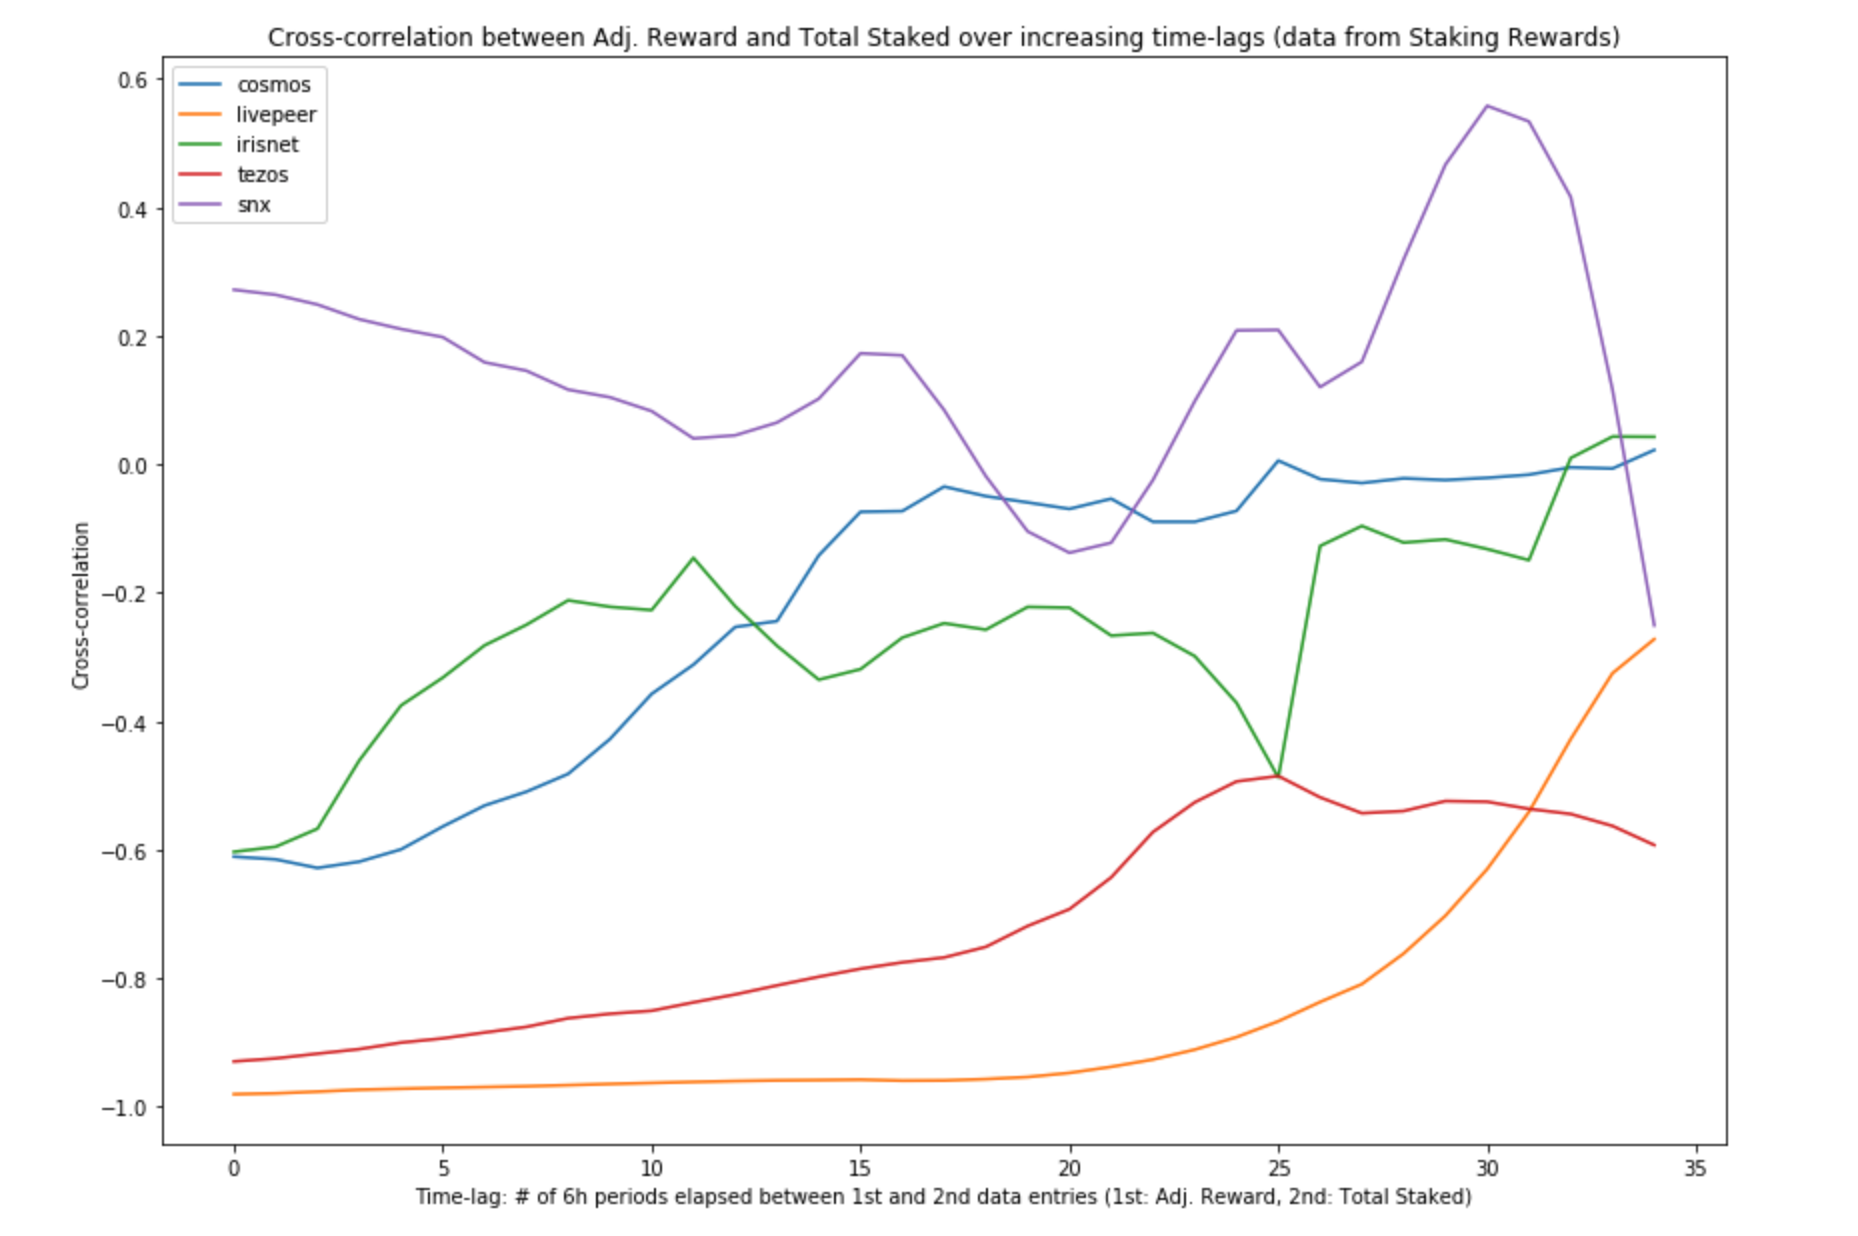
\includegraphics[width=\textwidth]{lagged_correlation_SR.png}
    \caption{Cross–correlation between Adjusted Reward and Total Staked over increasing time-lags. Data from Staking Rewards. N: [Cosmos: 1009, Livepeer: 1148, Irisnet: 1015, Tezos: 1371, SNX: 1005]. All five time series end in mid-February 2020.}
    \label{fig:tp}
\end{figure}

Thus, the notion that \textit{node operators can only be counted on for a reliable service if they're well compensated, or will quickly abandon the network} appears, so far, to be empirically false. None of the networks under examination, across multiple data set versions (from Staking Rewards and Staked Yields), have experienced a shortfall of operators, nor are there any observable trends that correlate decreasing earnings with a increasing paucity of supply, or increasing earnings with an increasing abundance of supply. There are multiple explanations for this, but none contradict the overarching rationale of this proposal. For example, one may study this seemingly unshakeable staker loyalty and tolerance of low reward rates, in the first year of these networks' existence and beyond, and attribute it to a prevalence of long-term investment strategies, deep pockets, ideological commitment or even irrational enthusiasm. Crucially, regardless of which underlying explanation you favour, there remains a strong case to flatten the minting schedule such that the earliest node operators do not capture a disproportionate share of the total supply.

\section{Deriving new parameters}

The previous draft inflation model utilizes the following parameters:
\begin{itemize}
    \item Genesis inflation rate – $I_0$ = 100\%
    \item Inflation rate half-life – $T_{1/2}$ = 2 years
    \item Genesis supply – $S_0$ = 1 billion tokens 
    \item Max tokens ever minted – $S(\infty)$ = 3.885 billion tokens
\end{itemize}
\\\\
In parametrizing the new, two-phase model, we choose to maintain certain parameters from the previous draft. We therefore derive a new genesis inflation rate such that the total number of tokens ever to be minted, $S(\infty)$, remains approximately 3.885 billion, and the half-life in the second phase, $T_{1/2}$, remains 2 years. This means that the number of tokens minted in the the first five years is necessarily lower than in the previous draft. 
\\\\
We can derive the new genesis inflation rate – $I_{static}$ – using an expression for the total supply at $t=\infty$ , which is the sum of (1) the tokens circulating at genesis, (2) the tokens minted in the first phase, and (3) the tokens minted in the second phase. Note that the boundaries of the second integral are $0$ and $\infty$, rather than $5$ and $\infty$, because the second phase exists mathematically \textit{as though} there was no first phase. Note also that all numerical figures in this derivation are rounded for readability.

\begin{equation}
    S(\infty) = S_0  +  S_0 \cdot \int_0^{5} I_{static}(t)\, dt  +  S_0 \cdot \int_0^{\infty} I_{static}(t)\, dt
\end{equation}

Tthe following equation calculates the decaying inflation rate at a time $t$.
 
 \begin{equation}
    I(t) = I_0 \cdot 2^{-\frac{t}{T_{1/2}}}
\end{equation}

We sub in $3.885 \cdot S_0$ for $S(\infty)$ and solve the first integral.

\begin{equation}
    3.885 \cdot S_0  = S_0 + S_0 \cdot (5 \cdot I_{static}) + S_0 \cdot \int_0^{\infty}     I_{static} \cdot 2^{-\frac{t}{T_{1/2}}} \, dt
\end{equation}

We cancel out $S_0$ and solve the second integral.

\begin{equation}
    3.885 = 1 + 5 \cdot  I_{static} + I_{static} \cdot \left[\frac{-2^{(1-\frac{t}{2})}}{\ln{2}}\right]_0^\infty
\end{equation}

We are now able to find an expression for $I_{static}$.

\begin{equation}
    2.885 = I_{static} \cdot (5 + \frac{2}{\ln{2}})
\end{equation}

\begin{equation}
   I_{static} = \frac{2.885}{7.885} = 36.6\%
\end{equation}

This is equivalent to a daily inflation rate of 0.10\% in the first five years, equivalent to the first 1826 periods.
\\\\
Note that the inflation rate of 0.10\% is applied, in each of the first 1825 periods, \textbf{to the genesis supply} ($S_0$ = 1 billion), not, as some may assume, to the variable supply ($S$ $>$ 1 billion). In other words, the supply grows by a constant number of tokens every period, which implies that the `real' percentage growth rate of the supply actually decreases period-to-period. 
\\\\
To avoid confusing the inflation rate with the real growth rate of the supply, we hereafter suggest the term \textit{minting schedule} to describe the growth of the circulating supply.
\\\\
So the minting schedule of the two-phase model, over the first five years, is as follows: 

\begin{equation}
   I_{static} \cdot S_0 = 365,915,960\:new \:tokens \:per \:year
\end{equation}
\\
This is equivalent to 1,002,509 newly minted tokens released into the circulating supply, every period for the first 1825 periods. 
\\\\
It's important to note that this distinction between the inflation rate and real growth rate of the supply is not a unique feature of the the two-phase proposal. In the previous draft model, the real growth rate of the supply decreases \textit{more rapidly} than the inflation rate – since it is a function of both the inflation rate's decay \textit{and} the supply's growth over time. This is particularly relevant because the second phase of the two-phase model follows a similar formula. The minting schedule after period 1825 (the last day of year 5) involves a rate which decays period-to-period, applied daily to the constant of the genesis supply (1 billion tokens). For example, 1,001,558 new tokens are minted on day 1827, which is 951 fewer than the previous day.
\\\\
With this new token minting schedule, we can work out that approximately 1.83 billion tokens are minted in the first 5 years, followed by approximately a further 1.056 billion between the fifth year and t = $\infty$.

\end{document}

In other words, the same amount of tokens will be emitted from $t=5$ until $t=\infty$ 

Similarly, the proposal does not cover the individual yield (the actual earnings of each staker, which is a function of the overall staking percentage and dilution), and focus this proposal on the \textit{nominal} inflation rate.